\documentclass[twoside]{book}

% Packages required by doxygen
\usepackage{fixltx2e}
\usepackage{calc}
\usepackage{doxygen}
\usepackage[export]{adjustbox} % also loads graphicx
\usepackage{graphicx}
\usepackage[utf8]{inputenc}
\usepackage{makeidx}
\usepackage{multicol}
\usepackage{multirow}
\PassOptionsToPackage{warn}{textcomp}
\usepackage{textcomp}
\usepackage[nointegrals]{wasysym}
\usepackage[table]{xcolor}

% Font selection
\usepackage[T1]{fontenc}
\usepackage[scaled=.90]{helvet}
\usepackage{courier}
\usepackage{amssymb}
\usepackage{sectsty}
\renewcommand{\familydefault}{\sfdefault}
\allsectionsfont{%
  \fontseries{bc}\selectfont%
  \color{darkgray}%
}
\renewcommand{\DoxyLabelFont}{%
  \fontseries{bc}\selectfont%
  \color{darkgray}%
}
\newcommand{\+}{\discretionary{\mbox{\scriptsize$\hookleftarrow$}}{}{}}

% Page & text layout
\usepackage{geometry}
\geometry{%
  a4paper,%
  top=2.5cm,%
  bottom=2.5cm,%
  left=2.5cm,%
  right=2.5cm%
}
\tolerance=750
\hfuzz=15pt
\hbadness=750
\setlength{\emergencystretch}{15pt}
\setlength{\parindent}{0cm}
\setlength{\parskip}{0.2cm}
\makeatletter
\renewcommand{\paragraph}{%
  \@startsection{paragraph}{4}{0ex}{-1.0ex}{1.0ex}{%
    \normalfont\normalsize\bfseries\SS@parafont%
  }%
}
\renewcommand{\subparagraph}{%
  \@startsection{subparagraph}{5}{0ex}{-1.0ex}{1.0ex}{%
    \normalfont\normalsize\bfseries\SS@subparafont%
  }%
}
\makeatother

% Headers & footers
\usepackage{fancyhdr}
\pagestyle{fancyplain}
\fancyhead[LE]{\fancyplain{}{\bfseries\thepage}}
\fancyhead[CE]{\fancyplain{}{}}
\fancyhead[RE]{\fancyplain{}{\bfseries\leftmark}}
\fancyhead[LO]{\fancyplain{}{\bfseries\rightmark}}
\fancyhead[CO]{\fancyplain{}{}}
\fancyhead[RO]{\fancyplain{}{\bfseries\thepage}}
\fancyfoot[LE]{\fancyplain{}{}}
\fancyfoot[CE]{\fancyplain{}{}}
\fancyfoot[RE]{\fancyplain{}{\bfseries\scriptsize Generated on Tue Oct 27 2015 10\+:32\+:22 for Quantum Phase Estimation with Reinforcement Learning by Doxygen }}
\fancyfoot[LO]{\fancyplain{}{\bfseries\scriptsize Generated on Tue Oct 27 2015 10\+:32\+:22 for Quantum Phase Estimation with Reinforcement Learning by Doxygen }}
\fancyfoot[CO]{\fancyplain{}{}}
\fancyfoot[RO]{\fancyplain{}{}}
\renewcommand{\footrulewidth}{0.4pt}
\renewcommand{\chaptermark}[1]{%
  \markboth{#1}{}%
}
\renewcommand{\sectionmark}[1]{%
  \markright{\thesection\ #1}%
}

% Indices & bibliography
\usepackage{natbib}
\usepackage[titles]{tocloft}
\setcounter{tocdepth}{3}
\setcounter{secnumdepth}{5}
\makeindex

% Hyperlinks (required, but should be loaded last)
\usepackage{ifpdf}
\ifpdf
  \usepackage[pdftex,pagebackref=true]{hyperref}
\else
  \usepackage[ps2pdf,pagebackref=true]{hyperref}
\fi
\hypersetup{%
  colorlinks=true,%
  linkcolor=blue,%
  citecolor=blue,%
  unicode%
}

% Custom commands
\newcommand{\clearemptydoublepage}{%
  \newpage{\pagestyle{empty}\cleardoublepage}%
}


%===== C O N T E N T S =====

\begin{document}

% Titlepage & ToC
\hypersetup{pageanchor=false,
             bookmarks=true,
             bookmarksnumbered=true,
             pdfencoding=unicode
            }
\pagenumbering{roman}
\begin{titlepage}
\vspace*{7cm}
\begin{center}%
{\Large Quantum Phase Estimation with Reinforcement Learning \\[1ex]\large 0.\+1 }\\
\vspace*{1cm}
{\large Generated by Doxygen 1.8.10}\\
\vspace*{0.5cm}
{\small Tue Oct 27 2015 10:32:22}\\
\end{center}
\end{titlepage}
\clearemptydoublepage
\tableofcontents
\clearemptydoublepage
\pagenumbering{arabic}
\hypersetup{pageanchor=true}

%--- Begin generated contents ---
\chapter{Main Page}
\label{index}\hypertarget{index}{}This project aims to show the use of reinforcement learning algorithm in finding a feedback policy for adaptive quantum-\/enhanced measurement, which has the goal of achieving the scaling in precision that exceeds the conventional techniques. We use adaptive phase estimation that includes phase noise and loss as the test problem.

The program is designed to streamline the implementation of population-\/based optimization algorithms on high-\/performance computing clusters and support parallel computing using M\+P\+I.

{\bfseries Features\+:}


\begin{DoxyItemize}
\item Easy selection of optimization algorithm and optimization problem
\item Libraries for differential evolution and particle swarm optimization
\item Both uniformly random and clustered initialization of population
\item Accept-\/reject criteria to ensure quantum-\/enhanced results
\item Support for V\+S\+L and G\+P\+U to provide fast random number generation
\end{DoxyItemize}

{\bfseries Limitation}

-\/\+The adaptive phase estimation is only reliable to 100 photons \mbox{[}Other limitation?\mbox{]}

\subsubsection*{Usage\+:}

As the program is designed to work on H\+P\+C clusters where interactive input from user might not be allowed, all the parameters are set within the code before compilation.

\paragraph*{Selecting problem and optimization algorithm}

The library for the optimization algorithm and the problem must be included in the headers of main.\+cpp. The objects in the corresponding classes can be set in the main function as pointers.


\begin{DoxyCode}
1 #include "mpi\_de.h"
2 #include "mpi\_pso.h"
\end{DoxyCode}


The optimization algorithms are instantiated with default parameters which can be changed within the code. For example, for differential evolution\+:


\begin{DoxyCode}
1 ...
2 
3 DE(Problem<typeT> *problem\_ptr): F(0.1), Cr(0.6) \{
4 
5 ...
\end{DoxyCode}


The library also contain a function for changing the parameters during runtime\+:


\begin{DoxyCode}
1 void DE<typeT>::write\_param(double *param\_array) \{
2 ...
\end{DoxyCode}


\paragraph*{Parameters setting}

The beginning of the main function contains a set of parameters including


\begin{DoxyItemize}
\item the smallest (N\+\_\+begin) and the largest number of variables (N\+\_\+end).
\item number of variables where the program use cluster initialization around previous solution (N\+\_\+cut)
\item number of variables where accept-\/reject criteria starts (data\+\_\+end)
\item population size (pop\+\_\+size)
\item number of iterations (iter, iter\+\_\+begin)
\end{DoxyItemize}

\paragraph*{Compilation}

The project contains the support for compilation using Autotools, and has been tested using G\+N\+U Compile Chain (G\+C\+C) and Intel Compilers. Intel V\+S\+L library and G\+P\+U are automatically detected.

In the first compilation, first run autogen.\+sh in order to create missing files and generate the executable configure from configure.\+ac. Then run the executable to generate Makefile from Makefile.\+in. The code can now be compiled. The sequence of the commands are


\begin{DoxyCode}
1 ./autogen.sh
2 
3 ./configure
4 
5 make
\end{DoxyCode}


Any job submission command should be directed to run src/phase\+\_\+estimation. The solution from the run are in the output file output.\+dat, and the time taken to run the program for each number of variables is in the file time.\+dat.

\subsubsection*{Acknowledgement\+:}

The computational work was enabled in part by support provided by West\+Grid (www.\+westgrid.\+ca) and Calcul Quebec (www.\+calculquebec.\+ca) through Compute Canada Calcul Canada (www.\+computecanada.\+ca).

\mbox{[}Should we include the funding sources\+: N\+S\+E\+R\+C, A\+I\+T\+F\mbox{]}

\subsubsection*{References\+:}

\mbox{[}To be include\+: manuscript on arxiv and manual -- what should be in the manual?\mbox{]} 
\chapter{Hierarchical Index}
\section{Class Hierarchy}
This inheritance list is sorted roughly, but not completely, alphabetically\+:\begin{DoxyCompactList}
\item \contentsline{section}{Candidate$<$ type\+T $>$}{\pageref{classCandidate}}{}
\item \contentsline{section}{Candidate$<$ double $>$}{\pageref{classCandidate}}{}
\item \contentsline{section}{Opt\+Alg}{\pageref{classOptAlg}}{}
\begin{DoxyCompactList}
\item \contentsline{section}{D\+E}{\pageref{classDE}}{}
\item \contentsline{section}{P\+S\+O}{\pageref{classPSO}}{}
\end{DoxyCompactList}
\item \contentsline{section}{Problem}{\pageref{classProblem}}{}
\begin{DoxyCompactList}
\item \contentsline{section}{Phase}{\pageref{classPhase}}{}
\end{DoxyCompactList}
\item \contentsline{section}{Rng\+Base}{\pageref{classRngBase}}{}
\begin{DoxyCompactList}
\item \contentsline{section}{Rng\+Simple}{\pageref{classRngSimple}}{}
\item \contentsline{section}{Rng\+Vectorized}{\pageref{classRngVectorized}}{}
\end{DoxyCompactList}
\end{DoxyCompactList}

\chapter{Class Index}
\section{Class List}
Here are the classes, structs, unions and interfaces with brief descriptions\+:\begin{DoxyCompactList}
\item\contentsline{section}{\hyperlink{classCandidate}{Candidate$<$ type\+T $>$} }{\pageref{classCandidate}}{}
\item\contentsline{section}{\hyperlink{classDE}{D\+E} }{\pageref{classDE}}{}
\item\contentsline{section}{\hyperlink{classOptAlg}{Opt\+Alg} }{\pageref{classOptAlg}}{}
\item\contentsline{section}{\hyperlink{classPhase}{Phase} }{\pageref{classPhase}}{}
\item\contentsline{section}{\hyperlink{classProblem}{Problem} }{\pageref{classProblem}}{}
\item\contentsline{section}{\hyperlink{classPSO}{P\+S\+O} }{\pageref{classPSO}}{}
\item\contentsline{section}{\hyperlink{classRngBase}{Rng\+Base} }{\pageref{classRngBase}}{}
\item\contentsline{section}{\hyperlink{classRngSimple}{Rng\+Simple} }{\pageref{classRngSimple}}{}
\item\contentsline{section}{\hyperlink{classRngVectorized}{Rng\+Vectorized} }{\pageref{classRngVectorized}}{}
\end{DoxyCompactList}

\chapter{Class Documentation}
\hypertarget{classCandidate}{}\section{Candidate$<$ type\+T $>$ Class Template Reference}
\label{classCandidate}\index{Candidate$<$ type\+T $>$@{Candidate$<$ type\+T $>$}}
\subsection*{Public Member Functions}
\begin{DoxyCompactItemize}
\item 
\hypertarget{classCandidate_a7d6563ae2246654a7b3e4c34a8f38e7f}{}void {\bfseries init\+\_\+can} (int numvar, int fit\+\_\+size)\label{classCandidate_a7d6563ae2246654a7b3e4c34a8f38e7f}

\item 
\hypertarget{classCandidate_adb4ae80a8dc02e8cb85df4d8c651d53c}{}void {\bfseries init\+\_\+velocity} ()\label{classCandidate_adb4ae80a8dc02e8cb85df4d8c651d53c}

\item 
\hypertarget{classCandidate_abc542c3e498ddc6e1bbf016c28ba035a}{}void {\bfseries update\+\_\+cont} (type\+T $\ast$input)\label{classCandidate_abc542c3e498ddc6e1bbf016c28ba035a}

\item 
\hypertarget{classCandidate_a66100c3779eadc81ab5bacbd4fe1d4b7}{}void {\bfseries update\+\_\+vel} (type\+T $\ast$input)\label{classCandidate_a66100c3779eadc81ab5bacbd4fe1d4b7}

\item 
\hypertarget{classCandidate_a60027d49ca1f7684245a0f9fe2864f30}{}void {\bfseries update\+\_\+best} ()\label{classCandidate_a60027d49ca1f7684245a0f9fe2864f30}

\item 
\hypertarget{classCandidate_abccd308b73aab3dd6c6403269fff2e66}{}void {\bfseries update\+\_\+global} (type\+T $\ast$input)\label{classCandidate_abccd308b73aab3dd6c6403269fff2e66}

\item 
\hypertarget{classCandidate_a68623f87b2353804a936704983de417f}{}void {\bfseries put\+\_\+to\+\_\+global} ()\label{classCandidate_a68623f87b2353804a936704983de417f}

\item 
\hypertarget{classCandidate_a5f781b1a2e563492fb33449df4196897}{}void {\bfseries read\+\_\+cont} (type\+T $\ast$output)\label{classCandidate_a5f781b1a2e563492fb33449df4196897}

\item 
\hypertarget{classCandidate_a49f8e0f5b9a3ad4df2993ef2415552ce}{}void {\bfseries read\+\_\+vel} (type\+T $\ast$output)\label{classCandidate_a49f8e0f5b9a3ad4df2993ef2415552ce}

\item 
\hypertarget{classCandidate_adc8885a1bc7990d5060fb41fb0b84307}{}void {\bfseries read\+\_\+best} (type\+T $\ast$output)\label{classCandidate_adc8885a1bc7990d5060fb41fb0b84307}

\item 
\hypertarget{classCandidate_ad8df30af1e76d0cbcc6563107877756e}{}void {\bfseries read\+\_\+global} (type\+T $\ast$output)\label{classCandidate_ad8df30af1e76d0cbcc6563107877756e}

\item 
\hypertarget{classCandidate_afe7099f234d4aab5f01bce84601dc19d}{}void {\bfseries write\+\_\+contfit} (double $\ast$fit, int tt)\label{classCandidate_afe7099f234d4aab5f01bce84601dc19d}

\item 
\hypertarget{classCandidate_a5d186a93dad0f8b333c8dadc86bdb1e2}{}void {\bfseries write\+\_\+bestfit} (double $\ast$fit)\label{classCandidate_a5d186a93dad0f8b333c8dadc86bdb1e2}

\item 
\hypertarget{classCandidate_a4eefbfbed65c2023619863de995333b6}{}void {\bfseries write\+\_\+globalfit} (double $\ast$fit)\label{classCandidate_a4eefbfbed65c2023619863de995333b6}

\item 
\hypertarget{classCandidate_a6baad7d2a8970192a5b4f1e148cfd907}{}double {\bfseries read\+\_\+contfit} (int i)\label{classCandidate_a6baad7d2a8970192a5b4f1e148cfd907}

\item 
\hypertarget{classCandidate_a87732e684af19e231b40f7556e3519a1}{}double {\bfseries read\+\_\+bestfit} (int i)\label{classCandidate_a87732e684af19e231b40f7556e3519a1}

\item 
\hypertarget{classCandidate_aa0c5b47e7e4f578b3661e641a9ddf9dd}{}double {\bfseries read\+\_\+globalfit} (int i)\label{classCandidate_aa0c5b47e7e4f578b3661e641a9ddf9dd}

\item 
\hypertarget{classCandidate_ad83fabe7087e40e18bb8d4d511abf67f}{}int {\bfseries read\+\_\+bestt} ()\label{classCandidate_ad83fabe7087e40e18bb8d4d511abf67f}

\end{DoxyCompactItemize}


The documentation for this class was generated from the following file\+:\begin{DoxyCompactItemize}
\item 
D\+:/\+In Work/\+Program/\+Git\+Hub/phase\+\_\+estimation/src/candidate.\+h\end{DoxyCompactItemize}

\hypertarget{classDE}{}\section{D\+E Class Reference}
\label{classDE}\index{D\+E@{D\+E}}
Inheritance diagram for D\+E\+:\begin{figure}[H]
\begin{center}
\leavevmode
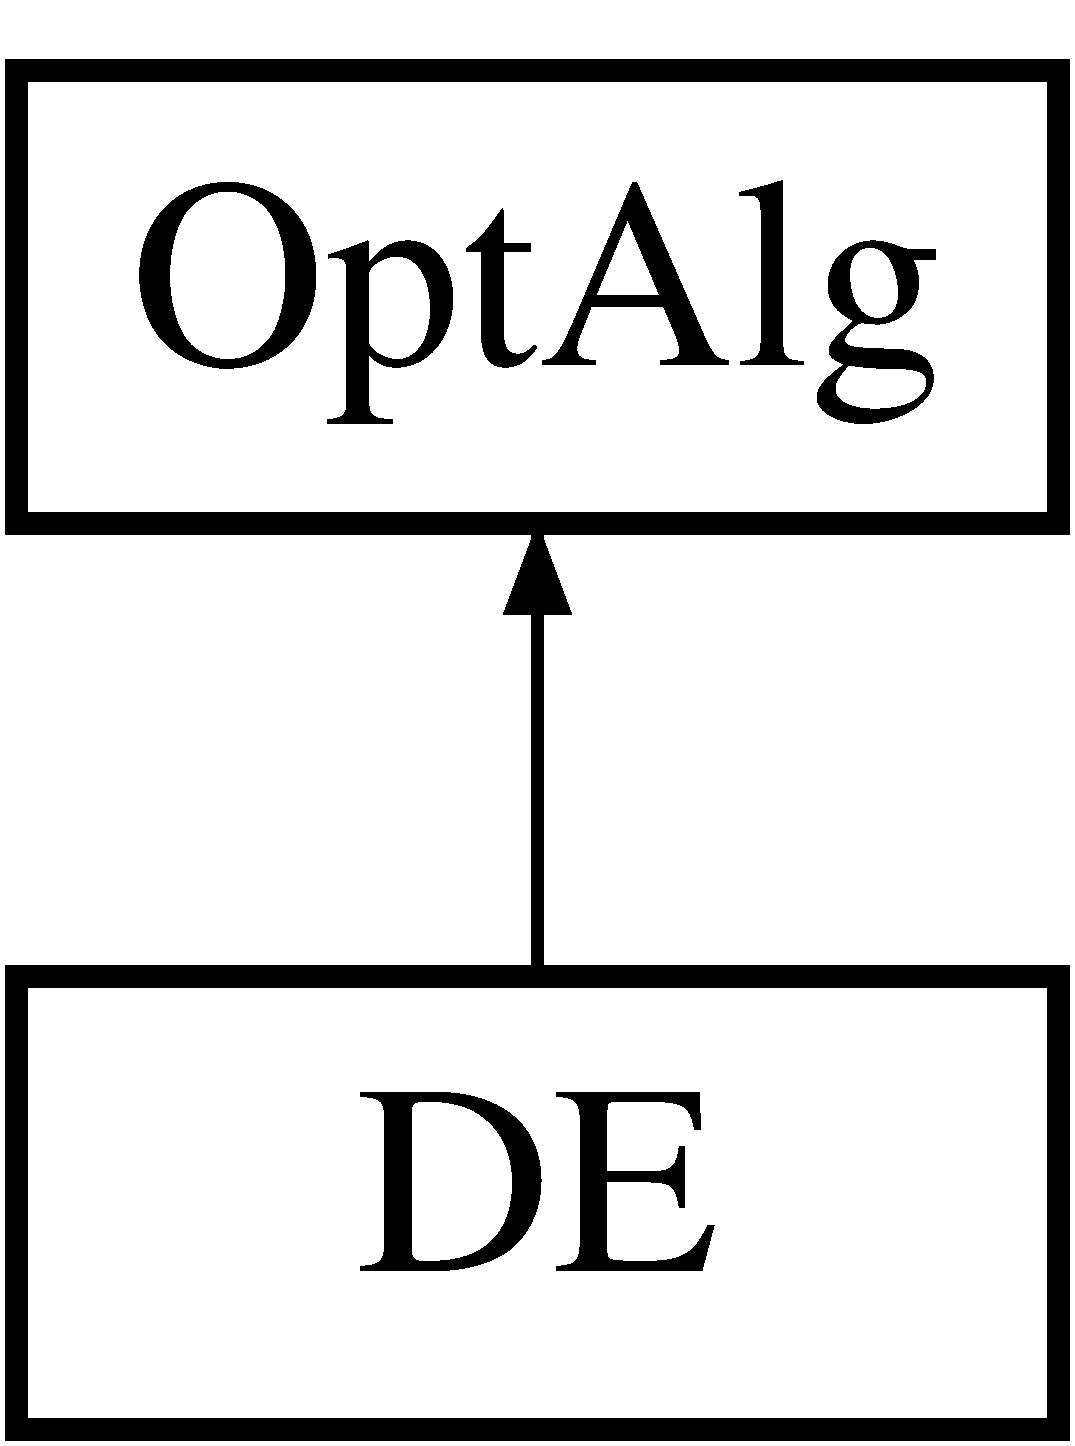
\includegraphics[height=2.000000cm]{classDE}
\end{center}
\end{figure}
\subsection*{Public Member Functions}
\begin{DoxyCompactItemize}
\item 
\hypertarget{classDE_a1f05cc6409494dee6f1a51f3b8fffb33}{}{\bfseries D\+E} (\hyperlink{classProblem}{Problem} $\ast$problem\+\_\+ptr)\label{classDE_a1f05cc6409494dee6f1a51f3b8fffb33}

\item 
\hypertarget{classDE_a2ff7cab053965600e264c8aaa20a5e98}{}void {\bfseries put\+\_\+to\+\_\+best} (int my\+\_\+rank, int total\+\_\+pop, int nb\+\_\+proc)\label{classDE_a2ff7cab053965600e264c8aaa20a5e98}

\item 
\hypertarget{classDE_a75bbf1f66249014230af0c36b1692da6}{}void {\bfseries combination} (int my\+\_\+rank, int total\+\_\+pop, int nb\+\_\+proc)\label{classDE_a75bbf1f66249014230af0c36b1692da6}

\item 
\hypertarget{classDE_aa7db64e161c9c0a8faa18fe54319f723}{}void {\bfseries selection} (int my\+\_\+rank, int total\+\_\+pop, int nb\+\_\+proc)\label{classDE_aa7db64e161c9c0a8faa18fe54319f723}

\item 
\hypertarget{classDE_a92e6613371643726878322829ce006e9}{}void {\bfseries fit\+\_\+to\+\_\+global} ()\label{classDE_a92e6613371643726878322829ce006e9}

\item 
\hypertarget{classDE_a2975856172cbfa1512919986dcf5a87f}{}void {\bfseries find\+\_\+global} (int my\+\_\+rank, int total\+\_\+pop, int nb\+\_\+proc)\label{classDE_a2975856172cbfa1512919986dcf5a87f}

\item 
\hypertarget{classDE_a07523caeeac589fc632a8aa87c8305dd}{}void {\bfseries write\+\_\+param} (double $\ast$param\+\_\+array)\label{classDE_a07523caeeac589fc632a8aa87c8305dd}

\item 
\hypertarget{classDE_a1ad5a8387091099c20f455ad30afb505}{}void {\bfseries read\+\_\+param} (double $\ast$param\+\_\+array)\label{classDE_a1ad5a8387091099c20f455ad30afb505}

\end{DoxyCompactItemize}
\subsection*{Additional Inherited Members}


The documentation for this class was generated from the following files\+:\begin{DoxyCompactItemize}
\item 
D\+:/\+In Work/\+Program/\+Git\+Hub/phase\+\_\+estimation/src/mpi\+\_\+optalg.\+h\item 
D\+:/\+In Work/\+Program/\+Git\+Hub/phase\+\_\+estimation/src/mpi\+\_\+de.\+cpp\end{DoxyCompactItemize}

\hypertarget{classOptAlg}{}\section{Opt\+Alg Class Reference}
\label{classOptAlg}\index{Opt\+Alg@{Opt\+Alg}}
Inheritance diagram for Opt\+Alg\+:\begin{figure}[H]
\begin{center}
\leavevmode
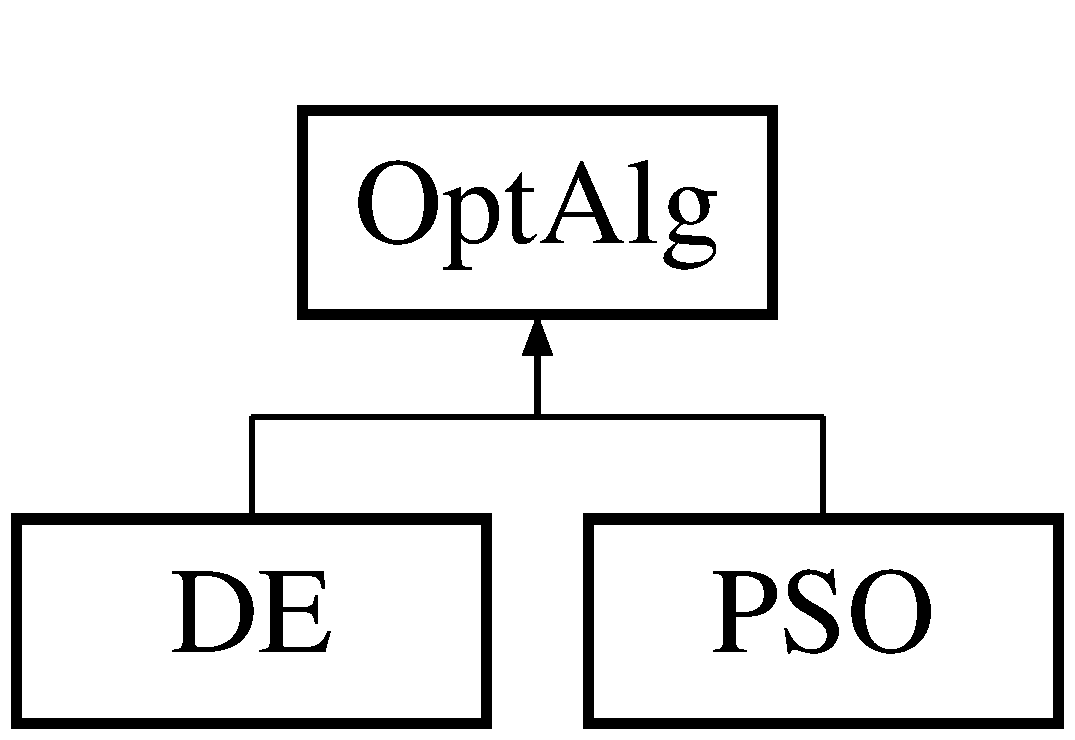
\includegraphics[height=2.000000cm]{classOptAlg}
\end{center}
\end{figure}
\subsection*{Public Member Functions}
\begin{DoxyCompactItemize}
\item 
\hypertarget{classOptAlg_abe77a22ec86aaf801f2050de5bdca121}{}{\bfseries Opt\+Alg} (\hyperlink{classProblem}{Problem} $\ast$problem\+\_\+ptr)\label{classOptAlg_abe77a22ec86aaf801f2050de5bdca121}

\item 
\hypertarget{classOptAlg_ac7569e761ec41dcbdad32af72f6a367c}{}virtual void {\bfseries put\+\_\+to\+\_\+best} (int my\+\_\+rank, int total\+\_\+pop, int nb\+\_\+proc)\label{classOptAlg_ac7569e761ec41dcbdad32af72f6a367c}

\item 
\hypertarget{classOptAlg_aa559fe662bf710dcb59fdbdad37d7166}{}virtual void {\bfseries combination} (int my\+\_\+rank, int total\+\_\+pop, int nb\+\_\+proc)\label{classOptAlg_aa559fe662bf710dcb59fdbdad37d7166}

\item 
\hypertarget{classOptAlg_a3badd6d65bfd2b578974fad574c54ce0}{}virtual void {\bfseries selection} (int my\+\_\+rank, int total\+\_\+pop, int nb\+\_\+proc)\label{classOptAlg_a3badd6d65bfd2b578974fad574c54ce0}

\item 
\hypertarget{classOptAlg_a30d9983af0d0eb8125e888e87fd37a99}{}virtual void {\bfseries write\+\_\+param} (double $\ast$param\+\_\+array)\label{classOptAlg_a30d9983af0d0eb8125e888e87fd37a99}

\item 
\hypertarget{classOptAlg_a7c1def4dcd71ac4a9f9b7edf06503557}{}virtual void {\bfseries read\+\_\+param} (double $\ast$param\+\_\+array)\label{classOptAlg_a7c1def4dcd71ac4a9f9b7edf06503557}

\item 
\hypertarget{classOptAlg_af9dd802bb54ddda92d1284ae1f9e03f8}{}virtual void {\bfseries fit\+\_\+to\+\_\+global} ()\label{classOptAlg_af9dd802bb54ddda92d1284ae1f9e03f8}

\item 
\hypertarget{classOptAlg_a5e29a74018889b754985e6e30cf0cd8a}{}virtual void {\bfseries find\+\_\+global} (int my\+\_\+rank, int total\+\_\+pop, int nb\+\_\+proc)\label{classOptAlg_a5e29a74018889b754985e6e30cf0cd8a}

\item 
\hypertarget{classOptAlg_aa41bb2ae61dade0b4a77ce73676b1e9e}{}void {\bfseries Init\+\_\+population} (int psize)\label{classOptAlg_aa41bb2ae61dade0b4a77ce73676b1e9e}

\item 
\hypertarget{classOptAlg_a492a3ed39231569801db4cf8f271da9f}{}void {\bfseries Init\+\_\+previous} (double prev\+\_\+dev, double new\+\_\+dev, int psize, double $\ast$prev\+\_\+soln)\label{classOptAlg_a492a3ed39231569801db4cf8f271da9f}

\item 
\hypertarget{classOptAlg_a777e1aa4c2eff276b03b1e68e0ae575e}{}void {\bfseries Cont\+\_\+fitness} (int p)\label{classOptAlg_a777e1aa4c2eff276b03b1e68e0ae575e}

\item 
\hypertarget{classOptAlg_a1bfdb110e81c3ecb852661df45abcaa8}{}void {\bfseries Best\+\_\+fitness} (int p)\label{classOptAlg_a1bfdb110e81c3ecb852661df45abcaa8}

\item 
\hypertarget{classOptAlg_a7db6fbc363c4d98858d7c10a60c26e96}{}void {\bfseries update\+\_\+popfit} ()\label{classOptAlg_a7db6fbc363c4d98858d7c10a60c26e96}

\item 
\hypertarget{classOptAlg_aede105b27f0777435108e3c8d79b0e91}{}void {\bfseries set\+\_\+success} (int iter, bool goal)\label{classOptAlg_aede105b27f0777435108e3c8d79b0e91}

\item 
\hypertarget{classOptAlg_a41481c4ce793a16e68a4d5950a9dfe48}{}bool {\bfseries check\+\_\+success} (int t, int D, double fit, double slope, double intercept)\label{classOptAlg_a41481c4ce793a16e68a4d5950a9dfe48}

\item 
\hypertarget{classOptAlg_ac6082918315a026c3d99c9e01b5820f7}{}double {\bfseries rand\+\_\+\+Gaussian} (double mean, double dev)\label{classOptAlg_ac6082918315a026c3d99c9e01b5820f7}

\item 
\hypertarget{classOptAlg_a066626a5ae556db202925836792d86af}{}void {\bfseries dev\+\_\+gen} (double $\ast$dev\+\_\+array, double prev\+\_\+dev, double new\+\_\+dev, int cut\+\_\+off)\label{classOptAlg_a066626a5ae556db202925836792d86af}

\item 
\hypertarget{classOptAlg_a6ea07ecb3d0dd5cbc13cd8b773c460c5}{}double {\bfseries Final\+\_\+select} (int my\+\_\+rank, int total\+\_\+pop, int nb\+\_\+proc, double $\ast$fit, double $\ast$solution, double $\ast$fitarray)\label{classOptAlg_a6ea07ecb3d0dd5cbc13cd8b773c460c5}

\item 
\hypertarget{classOptAlg_a99ec1f986f0b41c6d804d27ba6312b44}{}double {\bfseries avg\+\_\+\+Final\+\_\+select} (double $\ast$solution, int repeat, int my\+\_\+rank, int total\+\_\+pop, int nb\+\_\+proc, double $\ast$soln\+\_\+fit)\label{classOptAlg_a99ec1f986f0b41c6d804d27ba6312b44}

\item 
\hypertarget{classOptAlg_aeba3c4b026944928e9353ea49a3f2980}{}int {\bfseries find\+\_\+max} (double $\ast$fit, int total\+\_\+pop)\label{classOptAlg_aeba3c4b026944928e9353ea49a3f2980}

\item 
\hypertarget{classOptAlg_ab7f21c9001e6769c4505a6379f15590a}{}bool {\bfseries check\+\_\+policy} (double error, double sharp)\label{classOptAlg_ab7f21c9001e6769c4505a6379f15590a}

\item 
\hypertarget{classOptAlg_a41d6fd881634bf52b87bcaec6d210c44}{}void {\bfseries linear\+\_\+fit} (int data\+\_\+size, double $\ast$x, double $\ast$y, double $\ast$slope, double $\ast$intercept, double $\ast$mean\+\_\+x)\label{classOptAlg_a41d6fd881634bf52b87bcaec6d210c44}

\item 
\hypertarget{classOptAlg_a01eee569fc97269be39dee4d2b79bcb3}{}double {\bfseries error\+\_\+interval} (double $\ast$x, double $\ast$y, double mean\+\_\+x, int data\+\_\+size, double $\ast$S\+Sres, double slope, double intercept)\label{classOptAlg_a01eee569fc97269be39dee4d2b79bcb3}

\item 
\hypertarget{classOptAlg_ab4ba2cac1f5b51fb5fb715b780805825}{}double {\bfseries error\+\_\+update} (int old\+\_\+size, double $\ast$S\+Sres, double $\ast$mean\+\_\+x, double slope, double intercept, double $\ast$y, double $\ast$x)\label{classOptAlg_ab4ba2cac1f5b51fb5fb715b780805825}

\item 
\hypertarget{classOptAlg_a36a79062b361107b45689fecc4ad9585}{}double {\bfseries quantile} (double p)\label{classOptAlg_a36a79062b361107b45689fecc4ad9585}

\item 
\hypertarget{classOptAlg_abd15aea33f75b4da44eeea29bb553f82}{}double {\bfseries inv\+\_\+erf} (double x)\label{classOptAlg_abd15aea33f75b4da44eeea29bb553f82}

\item 
\hypertarget{classOptAlg_a38495fed6c3a7ed75df069109465f405}{}int {\bfseries sgn} (double x)\label{classOptAlg_a38495fed6c3a7ed75df069109465f405}

\end{DoxyCompactItemize}
\subsection*{Public Attributes}
\begin{DoxyCompactItemize}
\item 
\hypertarget{classOptAlg_ad83a3cc560bd483e499f26f629817f21}{}\hyperlink{classProblem}{Problem} $\ast$ {\bfseries prob}\label{classOptAlg_ad83a3cc560bd483e499f26f629817f21}

\item 
\hypertarget{classOptAlg_a2150acef11d441cb786afe578051e56f}{}bool {\bfseries success}\label{classOptAlg_a2150acef11d441cb786afe578051e56f}

\item 
\hypertarget{classOptAlg_ad269f7018945be9bdd6fb0237fb73c74}{}bool {\bfseries policy\+\_\+type}\label{classOptAlg_ad269f7018945be9bdd6fb0237fb73c74}

\item 
\hypertarget{classOptAlg_a90c8e3ad1c547ae5a8ee572b8f5aec98}{}int {\bfseries num}\label{classOptAlg_a90c8e3ad1c547ae5a8ee572b8f5aec98}

\item 
\hypertarget{classOptAlg_aad208e0441922169d0333c2277f1b7aa}{}int {\bfseries num\+\_\+fit}\label{classOptAlg_aad208e0441922169d0333c2277f1b7aa}

\end{DoxyCompactItemize}
\subsection*{Protected Attributes}
\begin{DoxyCompactItemize}
\item 
\hypertarget{classOptAlg_a3e8052f94b8cbecfe087377cc5c9a530}{}int {\bfseries pop\+\_\+size}\label{classOptAlg_a3e8052f94b8cbecfe087377cc5c9a530}

\item 
\hypertarget{classOptAlg_a9cbac99eb4f69fb2a3860ecec0dd3dc3}{}int {\bfseries T}\label{classOptAlg_a9cbac99eb4f69fb2a3860ecec0dd3dc3}

\item 
\hypertarget{classOptAlg_a716972bd2e408aa4b77be28fa2f0cbb1}{}int {\bfseries t}\label{classOptAlg_a716972bd2e408aa4b77be28fa2f0cbb1}

\item 
\hypertarget{classOptAlg_ae3e61ddad0b8f9a7170167852828c292}{}\hyperlink{classCandidate}{Candidate}$<$ double $>$ $\ast$ {\bfseries pop}\label{classOptAlg_ae3e61ddad0b8f9a7170167852828c292}

\item 
\hypertarget{classOptAlg_adf188f99e90b0d81c699dd5e8da9d93a}{}bool {\bfseries goal}\label{classOptAlg_adf188f99e90b0d81c699dd5e8da9d93a}

\end{DoxyCompactItemize}


The documentation for this class was generated from the following files\+:\begin{DoxyCompactItemize}
\item 
D\+:/\+In Work/\+Program/\+Git\+Hub/phase\+\_\+estimation/src/mpi\+\_\+optalg.\+h\item 
D\+:/\+In Work/\+Program/\+Git\+Hub/phase\+\_\+estimation/src/mpi\+\_\+optalg.\+cpp\end{DoxyCompactItemize}

\hypertarget{classPhase}{}\section{Phase Class Reference}
\label{classPhase}\index{Phase@{Phase}}
Inheritance diagram for Phase\+:\begin{figure}[H]
\begin{center}
\leavevmode
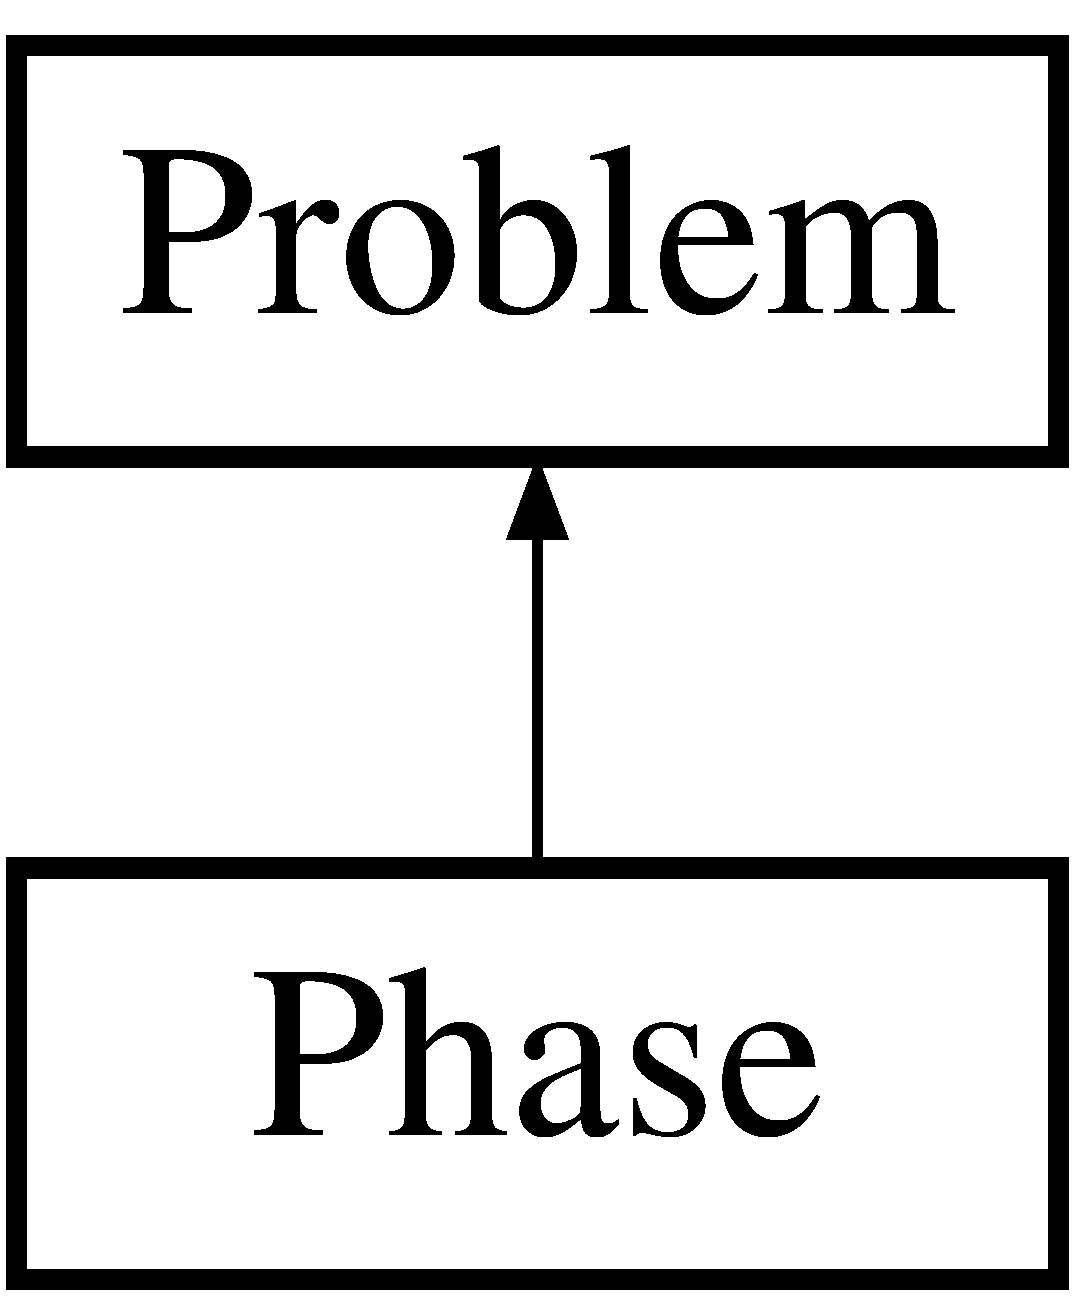
\includegraphics[height=2.000000cm]{classPhase}
\end{center}
\end{figure}
\subsection*{Public Member Functions}
\begin{DoxyCompactItemize}
\item 
\hypertarget{classPhase_a693a2d20b39fa8a91bf5f4c1afa3b2e2}{}{\bfseries Phase} (const int numvar, Rng $\ast$rng)\label{classPhase_a693a2d20b39fa8a91bf5f4c1afa3b2e2}

\item 
\hypertarget{classPhase_a73864e5e5e43b6fb301cf507eeb118a4}{}void {\bfseries avg\+\_\+fitness} (double $\ast$soln, const int K, double $\ast$fitarray)\label{classPhase_a73864e5e5e43b6fb301cf507eeb118a4}

\item 
\hypertarget{classPhase_a47d8ce9a16f64faa174dd69c3854e3e1}{}void {\bfseries boundary} (double $\ast$can1)\label{classPhase_a47d8ce9a16f64faa174dd69c3854e3e1}

\item 
\hypertarget{classPhase_a6100300c5e784c829375cceb5bf2de4c}{}void {\bfseries sqrtfac} (double $\ast$fac\+\_\+mat)\label{classPhase_a6100300c5e784c829375cceb5bf2de4c}

\item 
\hypertarget{classPhase_a3e758e9903183f98b634c09ec033517f}{}void {\bfseries one\+\_\+over\+\_\+fac} (double $\ast$over\+\_\+mat)\label{classPhase_a3e758e9903183f98b634c09ec033517f}

\item 
\hypertarget{classPhase_a386cfe3967d7b3cb11b66ded52237b85}{}double {\bfseries cal\+\_\+spart} (const int n, const int k, const int N)\label{classPhase_a386cfe3967d7b3cb11b66ded52237b85}

\item 
\hypertarget{classPhase_a58a0068df688f770ed388ad6bf63aa4f}{}void {\bfseries W\+K\+\_\+state} ()\label{classPhase_a58a0068df688f770ed388ad6bf63aa4f}

\item 
\hypertarget{classPhase_a6e2d1dd46651a342f46893d93c30041c}{}bool {\bfseries noise\+\_\+outcome} (const double phi, const double P\+H\+I, const int N)\label{classPhase_a6e2d1dd46651a342f46893d93c30041c}

\item 
\hypertarget{classPhase_a51090ea3a1cd12e9afd73faa48d04627}{}void {\bfseries state\+\_\+loss} (const int N)\label{classPhase_a51090ea3a1cd12e9afd73faa48d04627}

\item 
\hypertarget{classPhase_a395efd15826aac4793a6c37bf027825b}{}double {\bfseries mod\+\_\+2\+P\+I} (double P\+H\+I)\label{classPhase_a395efd15826aac4793a6c37bf027825b}

\end{DoxyCompactItemize}
\subsection*{Public Attributes}
\begin{DoxyCompactItemize}
\item 
\hypertarget{classPhase_a8b7dbdfafd0e3c84dba4138cace2e00b}{}double {\bfseries lower}\label{classPhase_a8b7dbdfafd0e3c84dba4138cace2e00b}

\item 
\hypertarget{classPhase_abe5215ac7a99447da0f2075e87b6e1d1}{}double {\bfseries upper}\label{classPhase_abe5215ac7a99447da0f2075e87b6e1d1}

\item 
\hypertarget{classPhase_a9508675d9cd23e96e4e5af0f3514d64e}{}double $\ast$ {\bfseries sqrt\+\_\+cache}\label{classPhase_a9508675d9cd23e96e4e5af0f3514d64e}

\item 
\hypertarget{classPhase_abcd241887b2113672f6dc94877b79079}{}Rng $\ast$ {\bfseries rng}\label{classPhase_abcd241887b2113672f6dc94877b79079}

\item 
\hypertarget{classPhase_a33f2132e12b166e3c7fe0059f67c71f9}{}dcmplx $\ast$ {\bfseries input\+\_\+state}\label{classPhase_a33f2132e12b166e3c7fe0059f67c71f9}

\item 
\hypertarget{classPhase_a64295bfa90607498ff8c544122afc3f9}{}double $\ast$ {\bfseries sqrtfac\+\_\+mat}\label{classPhase_a64295bfa90607498ff8c544122afc3f9}

\item 
\hypertarget{classPhase_a76beec42b9bfdcd105edcb8505bab934}{}double $\ast$ {\bfseries overfac\+\_\+mat}\label{classPhase_a76beec42b9bfdcd105edcb8505bab934}

\item 
\hypertarget{classPhase_a5ed12bc03ed5641e7d6486aefbc33ee3}{}double {\bfseries tan\+\_\+beta}\label{classPhase_a5ed12bc03ed5641e7d6486aefbc33ee3}

\item 
\hypertarget{classPhase_ab563c75af841b7c481f805d8a026518e}{}dcmplx $\ast$ {\bfseries state}\label{classPhase_ab563c75af841b7c481f805d8a026518e}

\item 
\hypertarget{classPhase_a29c2f7fd9df0afc222d810d037ea9ded}{}dcmplx $\ast$ {\bfseries update0}\label{classPhase_a29c2f7fd9df0afc222d810d037ea9ded}

\item 
\hypertarget{classPhase_aef5f586464d8609c933b2c28afc1fbf1}{}dcmplx $\ast$ {\bfseries update1}\label{classPhase_aef5f586464d8609c933b2c28afc1fbf1}

\end{DoxyCompactItemize}


The documentation for this class was generated from the following files\+:\begin{DoxyCompactItemize}
\item 
D\+:/\+In Work/\+Program/\+Git\+Hub/phase\+\_\+estimation/src/phase\+\_\+loss\+\_\+opt.\+h\item 
D\+:/\+In Work/\+Program/\+Git\+Hub/phase\+\_\+estimation/src/phase\+\_\+loss\+\_\+opt.\+cpp\end{DoxyCompactItemize}

\hypertarget{classProblem}{}\section{Problem Class Reference}
\label{classProblem}\index{Problem@{Problem}}
Inheritance diagram for Problem\+:\begin{figure}[H]
\begin{center}
\leavevmode
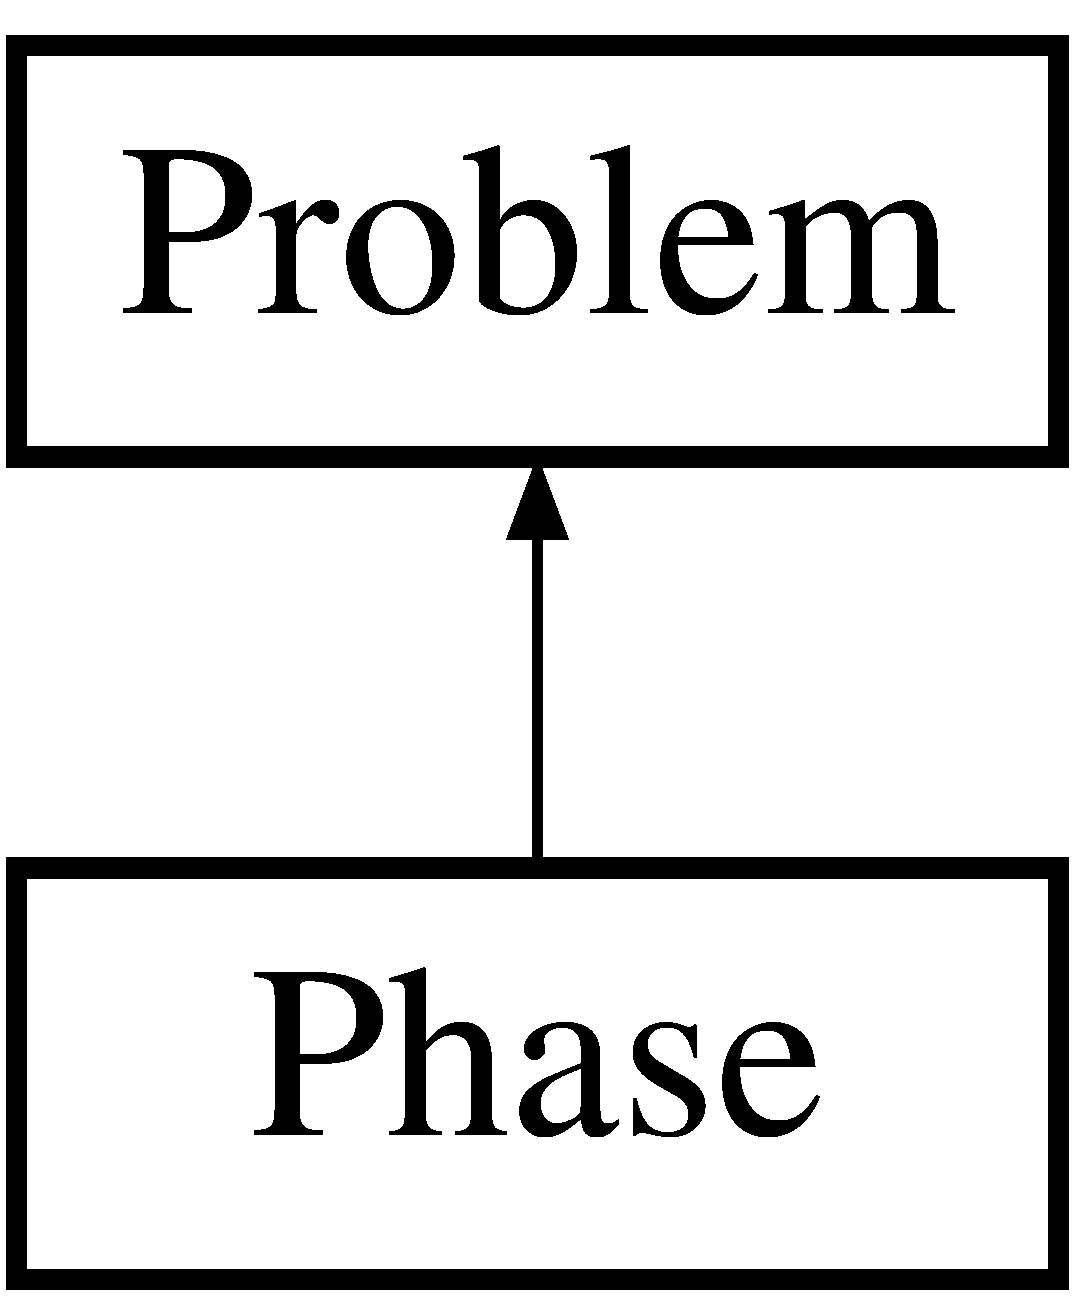
\includegraphics[height=2.000000cm]{classProblem}
\end{center}
\end{figure}
\subsection*{Public Member Functions}
\begin{DoxyCompactItemize}
\item 
\hypertarget{classProblem_a0109e1edec5b5b0fa682c5037132c308}{}virtual void {\bfseries fitness} (double $\ast$soln, double $\ast$fitarray)\label{classProblem_a0109e1edec5b5b0fa682c5037132c308}

\item 
\hypertarget{classProblem_a5a889257574b59d70c30e77f96657633}{}virtual void {\bfseries avg\+\_\+fitness} (double $\ast$soln, int K, double $\ast$fitarray)\label{classProblem_a5a889257574b59d70c30e77f96657633}

\item 
\hypertarget{classProblem_a866551d6c3a8c639eed39dd629459145}{}virtual void {\bfseries boundary} (double $\ast$can1)\label{classProblem_a866551d6c3a8c639eed39dd629459145}

\end{DoxyCompactItemize}
\subsection*{Public Attributes}
\begin{DoxyCompactItemize}
\item 
\hypertarget{classProblem_a4dfde0675e59264970f418516b799b2c}{}double $\ast$ {\bfseries lower\+\_\+bound}\label{classProblem_a4dfde0675e59264970f418516b799b2c}

\item 
\hypertarget{classProblem_a02bd6d1e098e211cc3bf0f5e02f20133}{}double $\ast$ {\bfseries upper\+\_\+bound}\label{classProblem_a02bd6d1e098e211cc3bf0f5e02f20133}

\item 
\hypertarget{classProblem_ae46e65561288cc81f06c2ddae062d303}{}int {\bfseries num}\label{classProblem_ae46e65561288cc81f06c2ddae062d303}

\item 
\hypertarget{classProblem_a02dc7cd36750260516f536d4b519399d}{}int {\bfseries num\+\_\+repeat}\label{classProblem_a02dc7cd36750260516f536d4b519399d}

\item 
\hypertarget{classProblem_a11dbb1d5a91b82ac8bab777362003e43}{}int {\bfseries num\+\_\+fit}\label{classProblem_a11dbb1d5a91b82ac8bab777362003e43}

\end{DoxyCompactItemize}


The documentation for this class was generated from the following file\+:\begin{DoxyCompactItemize}
\item 
D\+:/\+In Work/\+Program/\+Git\+Hub/phase\+\_\+estimation/src/problem.\+h\end{DoxyCompactItemize}

\hypertarget{classPSO}{}\section{P\+S\+O Class Reference}
\label{classPSO}\index{P\+S\+O@{P\+S\+O}}
Inheritance diagram for P\+S\+O\+:\begin{figure}[H]
\begin{center}
\leavevmode
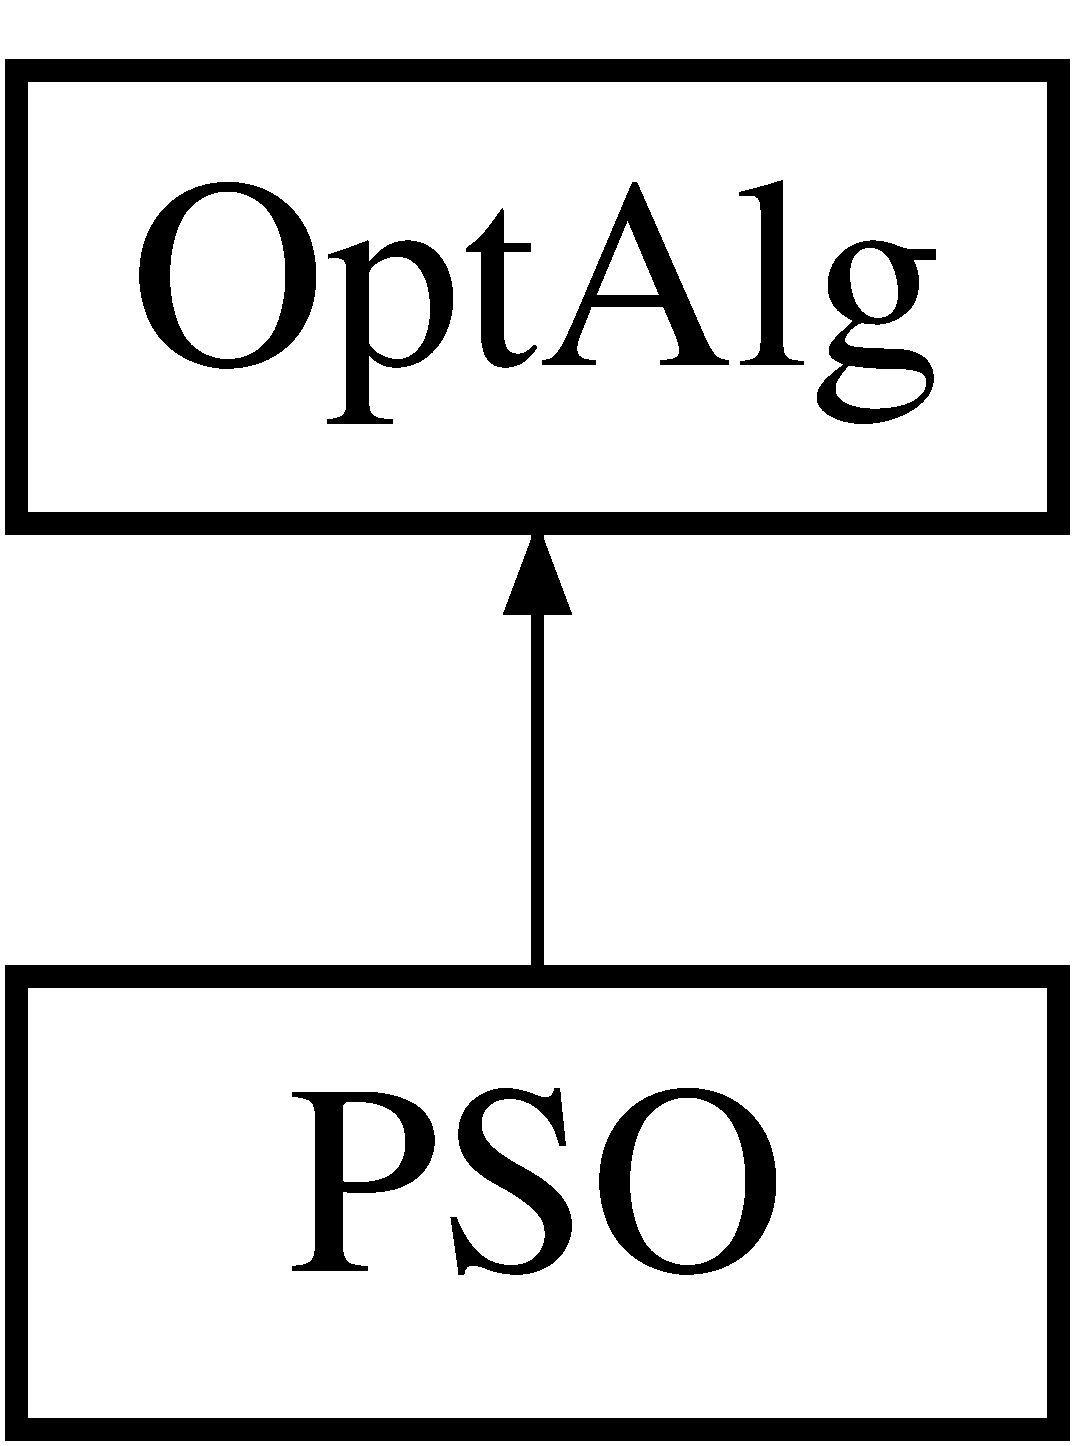
\includegraphics[height=2.000000cm]{classPSO}
\end{center}
\end{figure}
\subsection*{Public Member Functions}
\begin{DoxyCompactItemize}
\item 
\hypertarget{classPSO_a19611ceb537567770359bb5ab5c94071}{}{\bfseries P\+S\+O} (\hyperlink{classProblem}{Problem} $\ast$problem\+\_\+ptr)\label{classPSO_a19611ceb537567770359bb5ab5c94071}

\item 
\hypertarget{classPSO_a1222e7701e8e369a12d293afb16fb48c}{}void {\bfseries put\+\_\+to\+\_\+best} (int my\+\_\+rank, int total\+\_\+pop, int nb\+\_\+proc)\label{classPSO_a1222e7701e8e369a12d293afb16fb48c}

\item 
\hypertarget{classPSO_aa056f6a9f5ea1d916dbd425888084c3a}{}void {\bfseries combination} (int my\+\_\+rank, int total\+\_\+pop, int nb\+\_\+proc)\label{classPSO_aa056f6a9f5ea1d916dbd425888084c3a}

\item 
\hypertarget{classPSO_a4816c088f061f3089b350948d27f3707}{}void {\bfseries selection} (int my\+\_\+rank, int total\+\_\+pop, int nb\+\_\+proc)\label{classPSO_a4816c088f061f3089b350948d27f3707}

\item 
\hypertarget{classPSO_aa0b785a7ccee6b8b6e5d40d0c8100696}{}void {\bfseries write\+\_\+param} (double $\ast$param\+\_\+array)\label{classPSO_aa0b785a7ccee6b8b6e5d40d0c8100696}

\item 
\hypertarget{classPSO_a423f9f5a0a3b5ad7f1065e12ab050c0c}{}void {\bfseries read\+\_\+param} (double $\ast$param\+\_\+array)\label{classPSO_a423f9f5a0a3b5ad7f1065e12ab050c0c}

\item 
\hypertarget{classPSO_a17dedf795cd91539f2cf4c4f39f71938}{}void {\bfseries fit\+\_\+to\+\_\+global} ()\label{classPSO_a17dedf795cd91539f2cf4c4f39f71938}

\item 
\hypertarget{classPSO_a14fe336c8e970f1fdce9d91a36db3bb9}{}void {\bfseries find\+\_\+global} (int my\+\_\+rank, int total\+\_\+pop, int nb\+\_\+proc)\label{classPSO_a14fe336c8e970f1fdce9d91a36db3bb9}

\end{DoxyCompactItemize}
\subsection*{Additional Inherited Members}


The documentation for this class was generated from the following files\+:\begin{DoxyCompactItemize}
\item 
D\+:/\+In Work/\+Program/\+Git\+Hub/phase\+\_\+estimation/src/mpi\+\_\+optalg.\+h\item 
D\+:/\+In Work/\+Program/\+Git\+Hub/phase\+\_\+estimation/src/mpi\+\_\+pso.\+cpp\end{DoxyCompactItemize}

\hypertarget{classRngBase}{}\section{Rng\+Base Class Reference}
\label{classRngBase}\index{Rng\+Base@{Rng\+Base}}
Inheritance diagram for Rng\+Base\+:\begin{figure}[H]
\begin{center}
\leavevmode
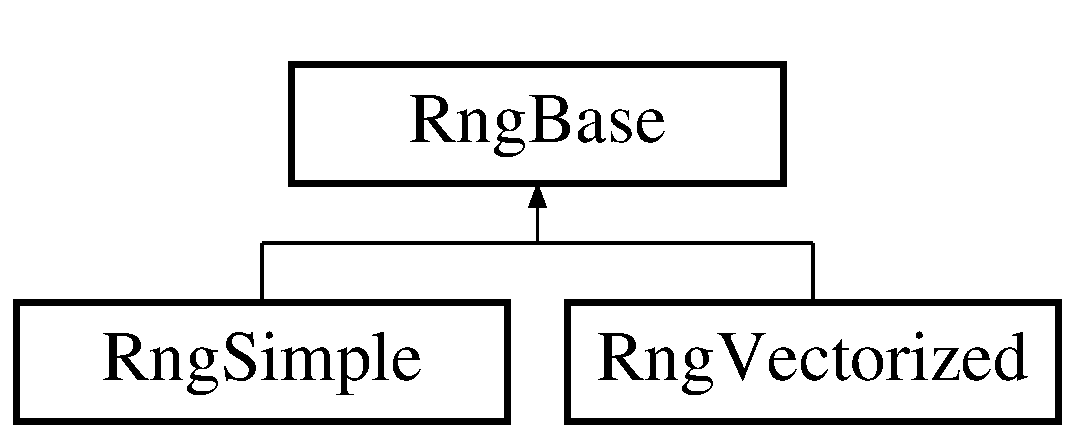
\includegraphics[height=2.000000cm]{classRngBase}
\end{center}
\end{figure}
\subsection*{Public Member Functions}
\begin{DoxyCompactItemize}
\item 
\hypertarget{classRngBase_ae40580575c22cfea7833aca8a17deacb}{}double {\bfseries next\+\_\+grand} (const double mean, const double dev)\label{classRngBase_ae40580575c22cfea7833aca8a17deacb}

\item 
\hypertarget{classRngBase_a0a9093fa49916814b2a30c5292663a65}{}double {\bfseries next\+\_\+urand} ()\label{classRngBase_a0a9093fa49916814b2a30c5292663a65}

\end{DoxyCompactItemize}


The documentation for this class was generated from the following file\+:\begin{DoxyCompactItemize}
\item 
D\+:/\+In Work/\+Program/\+Git\+Hub/phase\+\_\+estimation/src/rng.\+h\end{DoxyCompactItemize}

\hypertarget{classRngSimple}{}\section{Rng\+Simple Class Reference}
\label{classRngSimple}\index{Rng\+Simple@{Rng\+Simple}}
Inheritance diagram for Rng\+Simple\+:\begin{figure}[H]
\begin{center}
\leavevmode
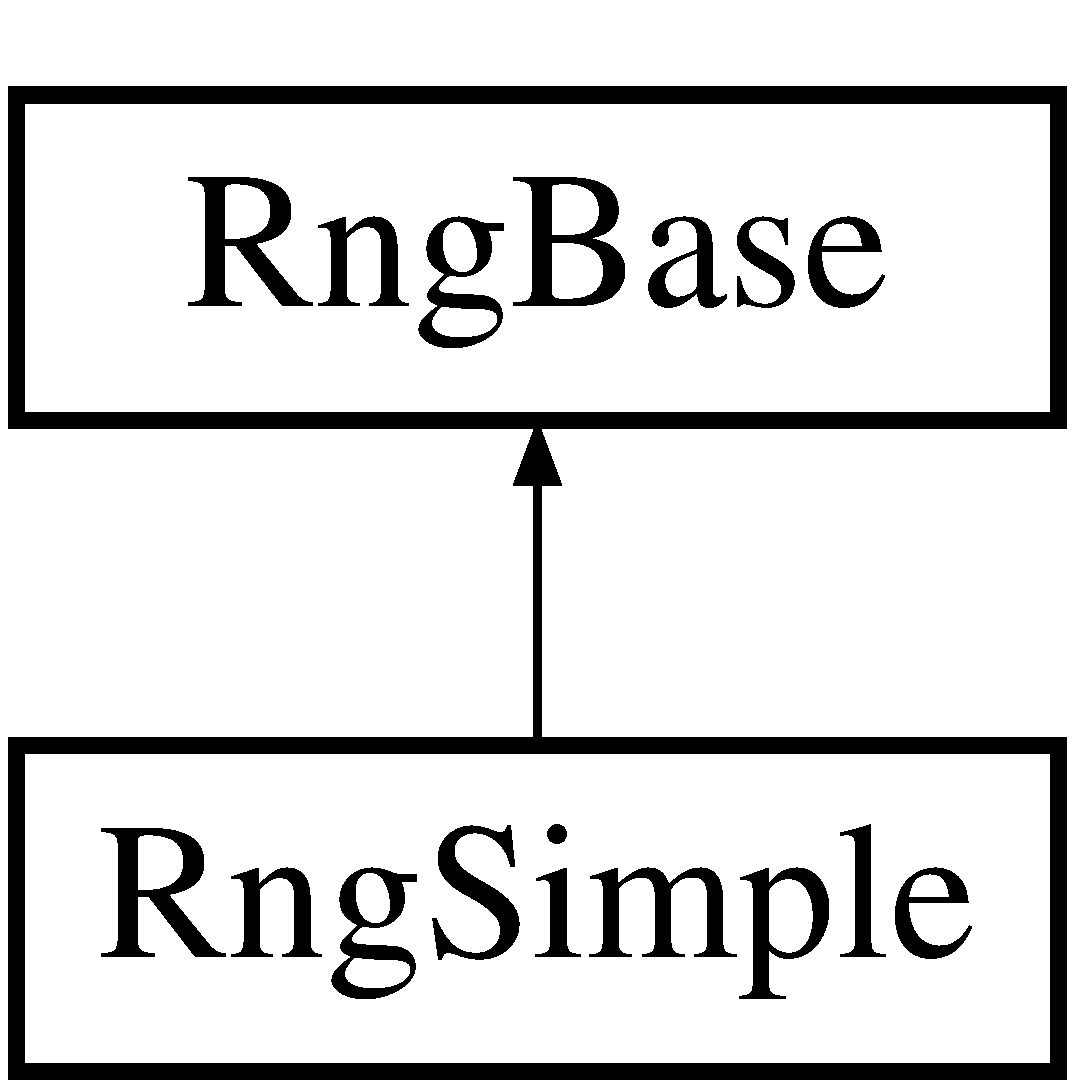
\includegraphics[height=2.000000cm]{classRngSimple}
\end{center}
\end{figure}
\subsection*{Public Member Functions}
\begin{DoxyCompactItemize}
\item 
\hypertarget{classRngSimple_a088385f8187d6f0ef7b38a39aa7340b4}{}{\bfseries Rng\+Simple} (int n\+\_\+urandom\+\_\+numbers, int n\+\_\+grandom\+\_\+numbers, int seed, int rank)\label{classRngSimple_a088385f8187d6f0ef7b38a39aa7340b4}

\item 
\hypertarget{classRngSimple_aba8d9e124fce30709c6056b50cd9dd5f}{}double {\bfseries next\+\_\+grand} (const double mean, const double dev)\label{classRngSimple_aba8d9e124fce30709c6056b50cd9dd5f}

\item 
\hypertarget{classRngSimple_a71c2deaf7fdf5c4f5379293021344aae}{}double {\bfseries next\+\_\+urand} ()\label{classRngSimple_a71c2deaf7fdf5c4f5379293021344aae}

\end{DoxyCompactItemize}


The documentation for this class was generated from the following files\+:\begin{DoxyCompactItemize}
\item 
D\+:/\+In Work/\+Program/\+Git\+Hub/phase\+\_\+estimation/src/rng.\+h\item 
D\+:/\+In Work/\+Program/\+Git\+Hub/phase\+\_\+estimation/src/rng.\+cpp\end{DoxyCompactItemize}

\hypertarget{classRngVectorized}{}\section{Rng\+Vectorized Class Reference}
\label{classRngVectorized}\index{Rng\+Vectorized@{Rng\+Vectorized}}
Inheritance diagram for Rng\+Vectorized\+:\begin{figure}[H]
\begin{center}
\leavevmode
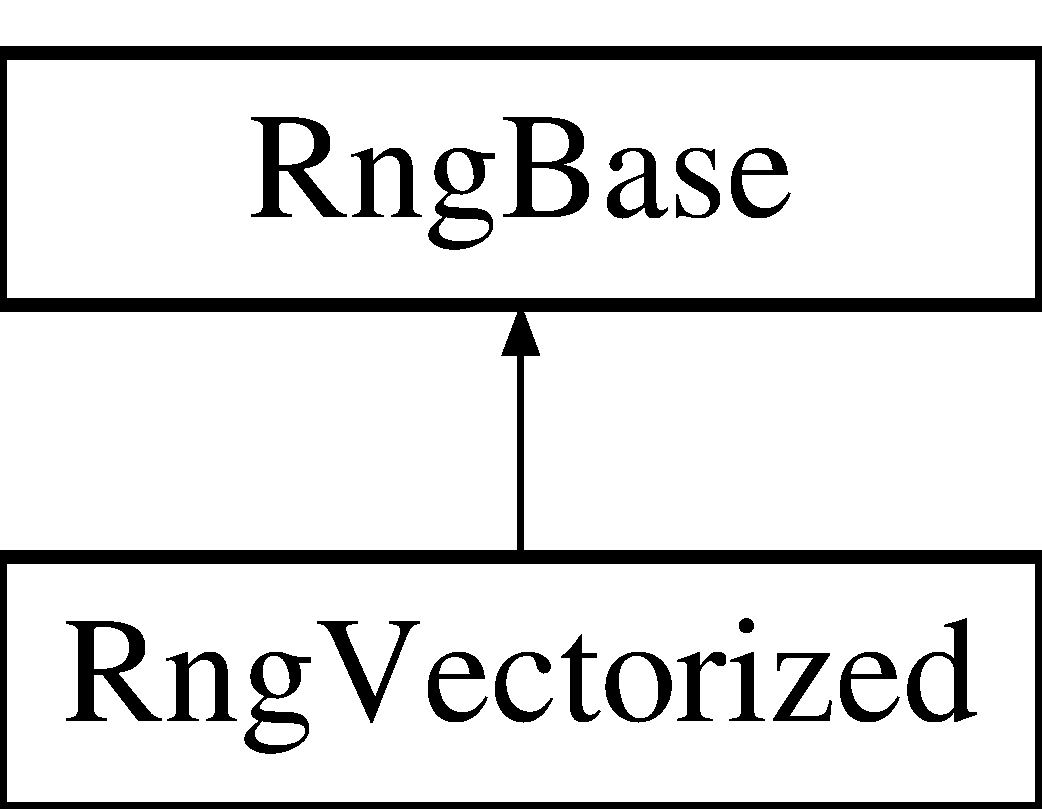
\includegraphics[height=2.000000cm]{classRngVectorized}
\end{center}
\end{figure}
\subsection*{Public Member Functions}
\begin{DoxyCompactItemize}
\item 
\hypertarget{classRngVectorized_a7a30dbbb27bd21f8d07731efd077a135}{}double {\bfseries next\+\_\+grand} (const double mean, const double dev)\label{classRngVectorized_a7a30dbbb27bd21f8d07731efd077a135}

\item 
\hypertarget{classRngVectorized_a82a1c6c3e3e70487e61c70c0c0920a34}{}double {\bfseries next\+\_\+urand} ()\label{classRngVectorized_a82a1c6c3e3e70487e61c70c0c0920a34}

\end{DoxyCompactItemize}


The documentation for this class was generated from the following file\+:\begin{DoxyCompactItemize}
\item 
D\+:/\+In Work/\+Program/\+Git\+Hub/phase\+\_\+estimation/src/rng.\+h\end{DoxyCompactItemize}

%--- End generated contents ---

% Index
\backmatter
\newpage
\phantomsection
\clearemptydoublepage
\addcontentsline{toc}{chapter}{Index}
\printindex

\end{document}
